\documentclass[conference]{IEEEtran}
% \documentclass[a4paper, 10pt, conference]{ieeeconf}
\IEEEoverridecommandlockouts
% The preceding line is only needed to identify funding in the first footnote. If that is unneeded, please comment it out.
%\usepackage{cite}
\usepackage{amsmath,amssymb,amsfonts, bm}
\usepackage{algorithmic}
\usepackage{graphicx}
\usepackage[backend=bibtex, sorting=none]{biblatex}
\addbibresource{references.bib}
\AtBeginBibliography{\scriptsize}
\usepackage{textcomp}
\usepackage{xcolor}
\usepackage{svg}
% \usepackage[svgnames]{xcolor}
% \usepackage[hidelinks]{hyperref}
% \usepackage[a-1b]{pdfx}
\providecommand{\keywords}[1]{\textbf{\textit{Index terms---}} #1}

\setsvg{
  inkscapeexe = {"C:/Program Files/Inkscape/bin/inkscape.exe"}
}
\def\BibTeX{{\rm B\kern-.05em{\sc i\kern-.025em b}\kern-.08em
    T\kern-.1667em\lower.7ex\hbox{E}\kern-.125emX}}
\begin{document}

\title{\LARGE \bf QP-based impact momentum maximization for a hammering task \\
                    by a humanoid robot
\thanks{}
}

\author{%
    Jimmy Vu$^{\dagger}$,
    Ruud Erens$^{\dagger}$,
    Hélène Stefanelli$^{\dagger}$$^{}$,
    Rafael Cisneros-Limón$^{\dagger}$$^{}$,
    Mehdi Benallegue$^{\dagger}$ \\
    and Abdelaziz Benallegue$^{\dagger}$%
    \thanks{$^
    {\dagger}$CNRS-AIST JRL (Joint Robotics Laboratory), IRL3218, 
    National Institute of Advanced Industrial Science and Technology (AIST), 
    Tsukuba, Japan. 
    Emails: 
    jimmyvu2016@yahoo.fr, 
    ruud.erens@solarteameindhoven.nl, 
    hstefanelli@student.ethz.ch, 
    rafael.cisneros@aist.go.jp, 
    mehdi.benallegue@aist.go.jp, 
    abdelaziz.benallegue@uvsq.fr
    }
    %
	%
}


\maketitle

\begin{abstract}
%Humanoid robots have the potential to relieve manual workers from wearing and exhausting tasks that may cause chronic joint damage over time.
Humanoid robots can offload repetitive, load-bearing operations that expose workers to cumulative joint stress.
In this paper, we focus on a hammering task with our humanoid robot HRP-5P and we propose a method to hit a nail with a given impact for a desired hitting velocity based on Quadratic Programming and the maximization of both the effective mass of the robot and impact momentum. 
Moreover, we implement a 5\textsuperscript{th} order Bézier curve as the trajectory, which ensures smooth, jerk-bounded motions from any reachable initial pose.
\end{abstract}

% \begin{keywords}
    \keywords{
quadratic programming, hammering, humanoid robot, effective mass, end-effector trajectory}
% \end{keywords}

\section{Introduction}
\noindent
Manual workers in physically difficult and wearing industries, such as the construction industry, have a 50\% higher risk of developing musculoskeletal disorders than people in other industries \cite{schneiderMusculoskeletalInjuriesConstruction2001}. 
Inadequate working posture and repetitive movements have been identified by Côté et al. \cite{coteDifferencesMultijointKinematic2005} to contribute to musculoskeletal disorders, which is the case for a hammering task. 
Furthermore, they demonstrated that fatigue affects elbow motion and shoulder injury affects both wrist and elbow motions during hammering. 
Balendra et al. \cite{balendraEffectHammerMass2017} showed that the increased moment exerted on joints during hammering can lead to more injuries, where a larger hammer causes a bigger increased moment. 
Unfortunately, larger hammers are often the preferred choice to accomplish such task.
Indeed, as a result from Petrič et al. \cite{petricHammeringDoesNot2017} indicates, hammers themselves are one of the non-powered handtools that cause the most injury \cite{aghazadehInjuriesDueHandtools1987}, especially to the fingers which are the most injured body part. 
Another cause of potential physical damage to workers is the posture that the hammering task has to be carried out with: Yuan-Ho Chen and Yi-Lang Chen \cite{chenOptimalEffectiveWorking2018} studied the optimal height to realize this task and concluded that it should be between 25 cm and 35 cm below the elbow height. 
However, it is not always possible to be at this height due to the variable working area in construction.

To relieve these workers from such joint-stressing activites, AIST developed the HRP-5P humanoid robot \cite{kanekoHumanoidRobotHRP5P2019} which can take care of the wearing and exhausting tasks, such as carrying heavy loads or hammering a nail,
the latter being the topic of this paper. 
Other impact tasks have been extensively studied: Cisneros et al. \cite{cisnerosImpulsivePedipulationSpherical2016} focused on impulsive pedipulation on a spherical object with a humanoid robot,
van Steen et al. \cite{steenRobotControlSimultaneous2022} proposed a control framework using Quadratic Programming (QP) to work with simultaneous impacts,
Tassi et al. \cite{tassiIMAcatcherIMpactawareNonprehensile2025} developed a method using velocity matching and a motion planner for catching high-impact flying objects to reduce hardware damage to the robot. 
Furthermore, Wang and Kheddar \cite{wangImpactFriendlyRobustControl2019} worked on robot damage mitigation by designing a conservative, robust and impact-friendly controller using QP.
Our overall objective is to hammer a target (a nail in our case) with the maximum impact and mitigate the recoil damage on the robot's joints.

This paper focuses on the impact maximization and the trajectory of the hammer tip to the nail using QP and a $5^{th}$ order Bézier curve.
Section \ref{Robot dynamic model} recalls the robot dynamic model that we use, 
in Section \ref{Impact modeling} we propose a model for the nail-hammer impact, 
Section \ref{Optimization of the effective mass using QP} details the usage of QP in our work to maximize the impact momentum, 
in Section \ref{Trajectory of the end-effector} we explain how to generate the trajectory of the end-effector to the nail, 
then we present simulations using the mc\_rtc framework \cite{mcrtc} in Section \ref{Simulations}, and finally we conclude our paper in Section \ref{Conclusion}.

\section{Robot dynamic model}
\label{Robot dynamic model}
\subsection{Robot dynamic equation}
\noindent
Let $n$ be the number of Degrees Of Freedom (DOF) of the humanoid robot. The dynamic equation of the robot writes:
\begin{equation}
    \mathbf{M(q) \ddot q} \, + \, \mathbf{C(q, \dot q) \dot q} \, + \, \mathbf{g(q)} = \mathbf{u} \, +  \sum_i \mathbf{J_i(q)^T F_i}
\label{RDE}
\end{equation}
where $\mathbf{q, \dot q, \ddot q} \in \mathbb{R}^n$ are the configuration, configuration velocity and configuration acceleration of the robot, respectively, $\mathbf{M(q)} \in \mathbb{R}^{n \times n}$ is the symmetric mass matrix or inertia matrix of the robot,
     $\mathbf{C(q, \dot q)} \in \mathbb{R}^{n \times n}$ is the dynamic factorization of the Coriolis matrix \cite{bjerkengNewCoriolisMatrix2012},
     $\mathbf{g(q)} \in \mathbb{R}^n $ is the vector of gravitational effects,
    % \item $\mathbf{\tau} \in \mathbb{R}^n $ is the vector of applied torques
     $\mathbf{u} \in \mathbb{R}^{n}$ is the input vector of torques,
     $\mathbf{F_i} \in \mathbb{R}^{6}$ is the vector of the $i$-th external wrench (or generalized forces), i.e. forces and torques on each axis, 
     $\mathbf{J_i(q)} \in \mathbb{R}^{6 \times n}$ is the absolute Jacobian of the point of application of $\mathbf{F_i}$, and $\{ \cdot \}^\mathbf{T}$ is the matrix transpose operator.
     
\subsection{Jacobian of the end-effector pose}
\noindent
Let $\mathbf{J} \in \mathbb{R}^{6 \times n}$ be the Jacobian matrix of the end-effector pose defined such that:
\begin{equation}
    \mathbf{\dot x} = \mathbf{J(q) \dot q} = \left[\mathbf{\dot x}_\nu^\mathbf{T} \ \ \ \mathbf{\dot x}_\omega^\mathbf{T} \right]^\mathbf{T}
\label{map xdot qdot}
\end{equation}
where $\mathbf{\dot x} \in \mathbb{R}^6$ is the task space velocity (translational and angular velocities) of the end-effector,  
% and the time derivative of the end-effector pose $\mathbf{x} \in \mathbb{R}^6$:
% \begin{equation}
%     \mathbf{x} = \left[\mathbf{x}_\nu^\mathbf{T} \ \ \ \mathbf{x}_\omega^\mathbf{T} \right]^\mathbf{T}
% \end{equation}
% where 
$\mathbf{\dot x}_\nu$, $\mathbf{\dot x}_\omega \in \mathbb{R}^3$ are the translational and angular part of $\mathbf{\dot x}$, respectively.

The $\mathbf{J}$ matrix can be computed using forward kinematics and written using two matrices $\mathbf{J}_\nu$, $\mathbf{J}_\omega \in \mathbb{R}^{3 \times n}$:
\begin{equation}
    \mathbf{J} = \frac{\partial \mathbf{x}}{ \partial \mathbf{q}} 
            =\left[\mathbf{J}_\nu^{\mathbf{T}} \ \ \ \mathbf{J}_\omega^{\mathbf{T}}\right]^{\mathbf{T}}
\end{equation}
where $\mathbf{J}_\nu$ is its translational part and $\mathbf{J}_\omega$ is its angular part.
\section{Impact modeling}
\label{Impact modeling}
\noindent
In this section, we propose a mathematical model of the impact between the hammer tip and the nail. This part is heavily inspired by Stronge \cite{STRONGE} and his particle impact model. 
\subsection{Common tangent plane of collision}
\noindent
In the sense of Stronge \cite{STRONGE}, we define the common tangent plane of collision as the plane passing through the contact point at the instant of collision that is tangent to both surfaces involved in the collision.
The normal unit vector to the collision $\mathbf{n} \in \mathbb{R}^3$ is defined as a vector orthogonal to that plane; see the schematic on Fig.~\ref{SCHEMATIC OF THE PROBLEM}.
% The schematic given by Fig.~\ref{Frames} displays the fixed world frame $w$, the hammer tip frame and the nail frame.
% \begin{figure}
%     \centering
%     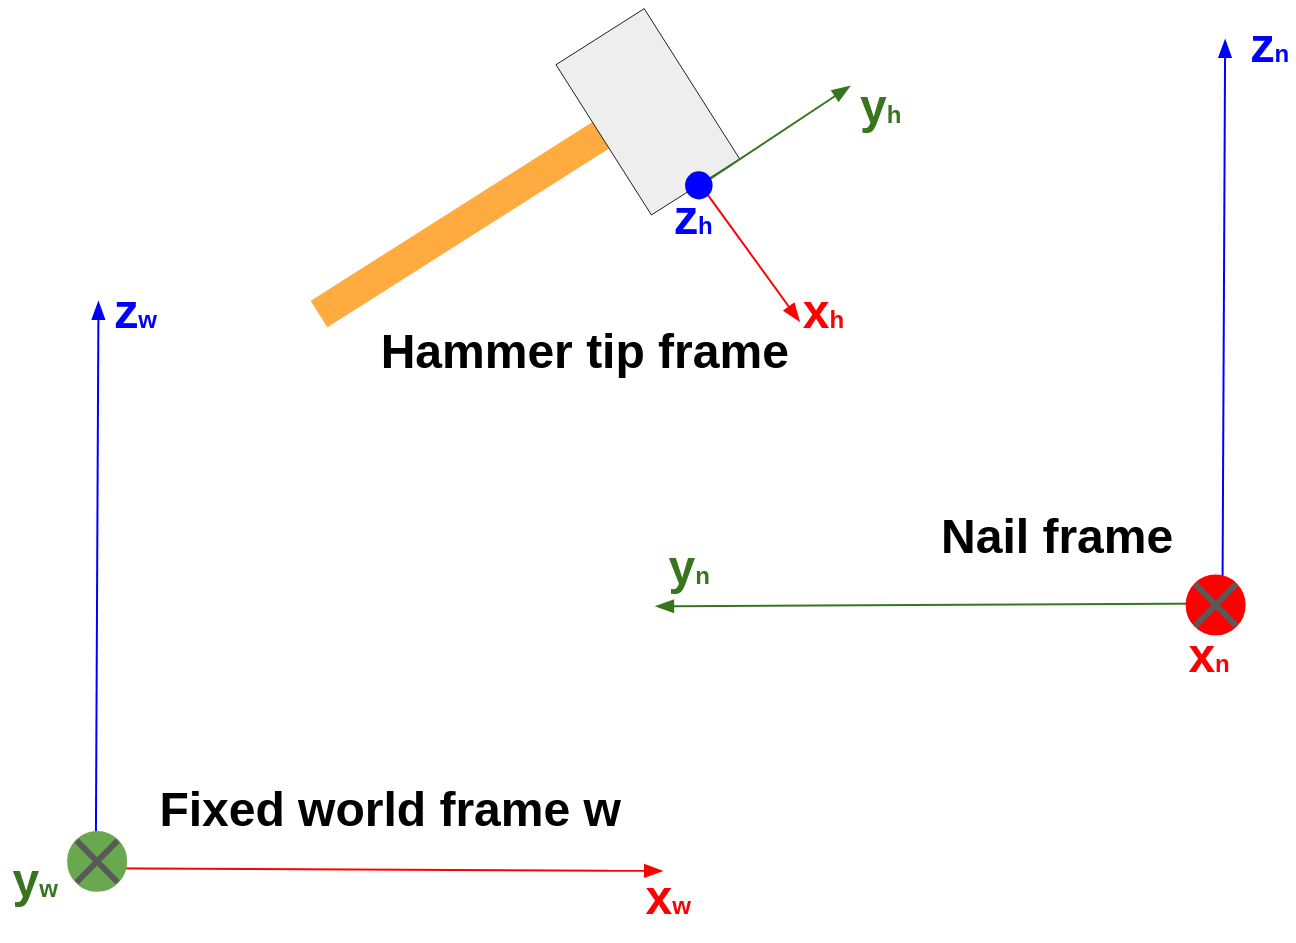
\includegraphics[width=0.85\linewidth]{Frames.png}
%     \caption{The fixed world frame $w$, hammer tip frame and nail frame}
%     \label{Frames}
% \end{figure}
% Without loss of generality, let's express $\mathbf{n}$ in the nail frame such that:\begin{equation}
%     \mathbf{n} = \left(0, 0, 1 \right)^{\mathbf{T}}
% \end{equation}

Let $\mathbf{R}_{w \to nail} \in SO(3)$ be the rotation matrix of the nail with respect to the world frame $w$. Then, the normal vector expressed in the world frame $\mathbf{n}_w$ is:
\begin{equation}
    \mathbf{n}_w = \mathbf{R}_{w \to nail}^{\mathbf{T}} \mathbf{n}
\end{equation}
\subsection{Effective mass of the robot}
\noindent
Let us define $m_{e,\mathbf{n}}(\mathbf{q}) \in \mathbb{R^+}$ (the ``e" stands for ``effective"), the configuration dependent Effective Mass of the Robot (EMR), as:
\begin{equation}
    m_{e,\mathbf{n}}(\mathbf{q}) \triangleq \left(\mathbf{n^T} \bm \Lambda (\mathbf{q}) \mathbf{n} \right)^{-1}
\label{effective mass}
\end{equation}
where $\bm \Lambda \in \mathbb{R}^{3 \times 3}$ is the mobility matrix \cite{cisnerosImpulsivePedipulationSpherical2016} defined as:
\begin{equation}
    \bm \Lambda(\mathbf{q}) \triangleq \mathbf{J_\nu(\mathbf{q}) M^{-1}(\mathbf{q})J_\nu^T(q)}
\end{equation}
The EMR represents the equivalent mass of the robot along the direction of $\mathbf{n}$ if we were to replace the robot by a particle.
\subsection{Choice of the model}
\noindent
We have three main ways to solve this impact problem: i) a force-based model, ii) an energy-based model and iii) a momentum-based model.

\subsubsection{Force-based model}
\noindent
The force-based model relies on Newton's second law:
\begin{equation}
    \mathbf{F}^h= m_{e,\mathbf{n}} \frac{d \mathbf{\dot x_\nu}}{dt}
\end{equation}
where $\mathbf{\dot x_{\nu}} \in \mathbb{R}^3$ is the translational part of $\mathbf{\dot x}$ defined in (\ref{map xdot qdot}), $\mathbf{F}^h \in \mathbb{R}^3$ is the force applied to the nail by the hammer (the superscript ``h" stands for ``hammer").
%  in the normal of the impact plane defined in (\ref{effective mass}). 
% The issue with this model is the well-definedness of the acceleration of the end-effector, which is the time derivative of $\mathbf{\dot x_\nu}$. 
The problem with this model is the discontinuous velocity of the hammer tip at the instant of collision, $t_c$, as the time derivative at this point in time does not exist. Therefore, we can not use a force-based model, except if we relax the instantanous nature of the impact model which is currently under study.
\\
\subsubsection{Energy-based model}
\label{Energy-based model}
\noindent
An energy-based model could be used to overcome the problem of discontinuity of the hammer tip velocity. 
However, during impact, the kinetic energy of the hammer tip is not fully transmitted to the nail: some of the energy is converted into heat, sound and deformation energy, which are difficult to estimate. 
Thus, although the model is still usable, we would have to estimate the losses, making the model less precise.
\\
\subsubsection{Momentum-based model}
\noindent
The momentum based model does not have the problems of the force-based model and the energy-based model. 
%Furthermore, another advantage of using this model is its ability to deal with discontinuous velocities, which occur when hitting a nail with a hammer. 
The main advantage of using this model is its ability to deal with discontinuous velocities, which occur when hitting a nail with a hammer. 
Furthermore, with momentum, the microscopic interactions between the hammer tip and the nail are taken into account through a scalar number $e_*$ called \textit{coefficient of restitution}, which measures the elasticity of the collision.
This coefficient can be used to study the post-impact dynamics of the colliding objects; however, this is out of the scope of this article and currently under study.
As such, we use the momentum model in the following part of the paper. 
More precisely, we use a model based on particle impact. A schematic depicting the problem is proposed in Fig.~\ref{SCHEMATIC OF THE PROBLEM}. 
In this model, an infinitesimal particle (i.e. with negligible size) models the local deformations of the hammer tip and the nail.

% \begin{figure*}
%     \centering
%     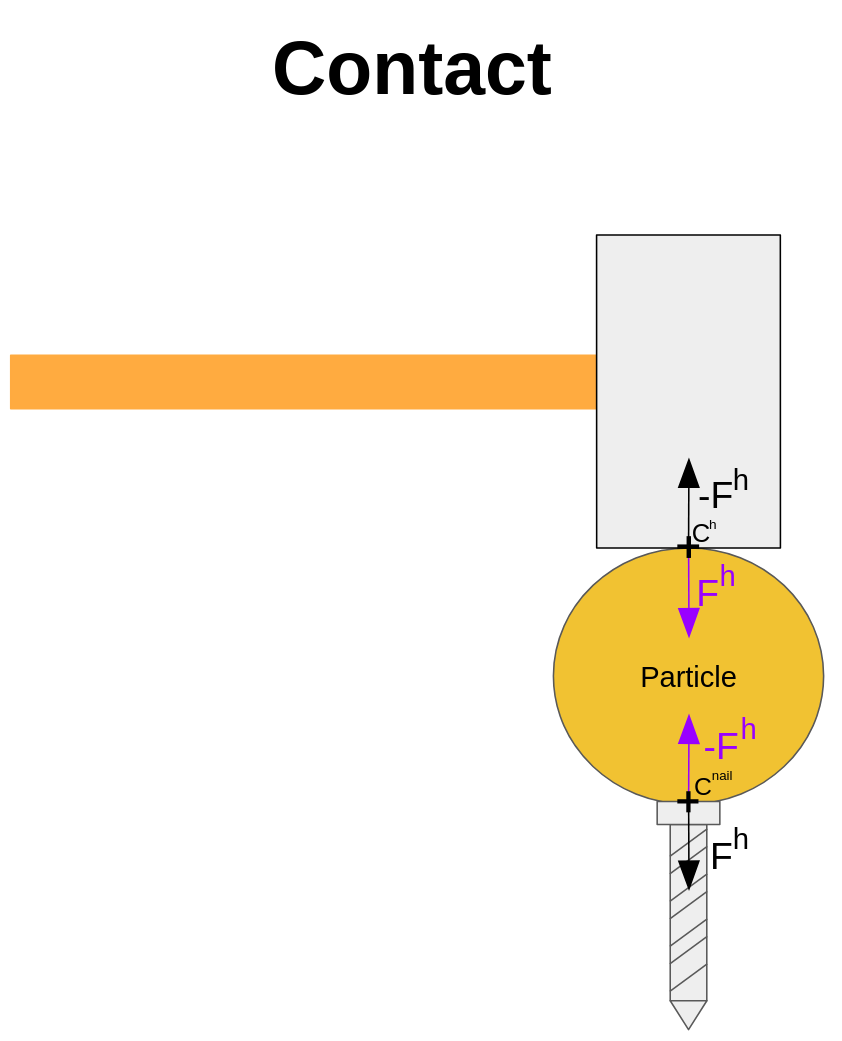
\includegraphics[width=0.5\linewidth]{Contact phase.png}
%     \caption{Contact is made between the particle and the hammer tip}
%     \label{CONTACT}
%     \centering
%     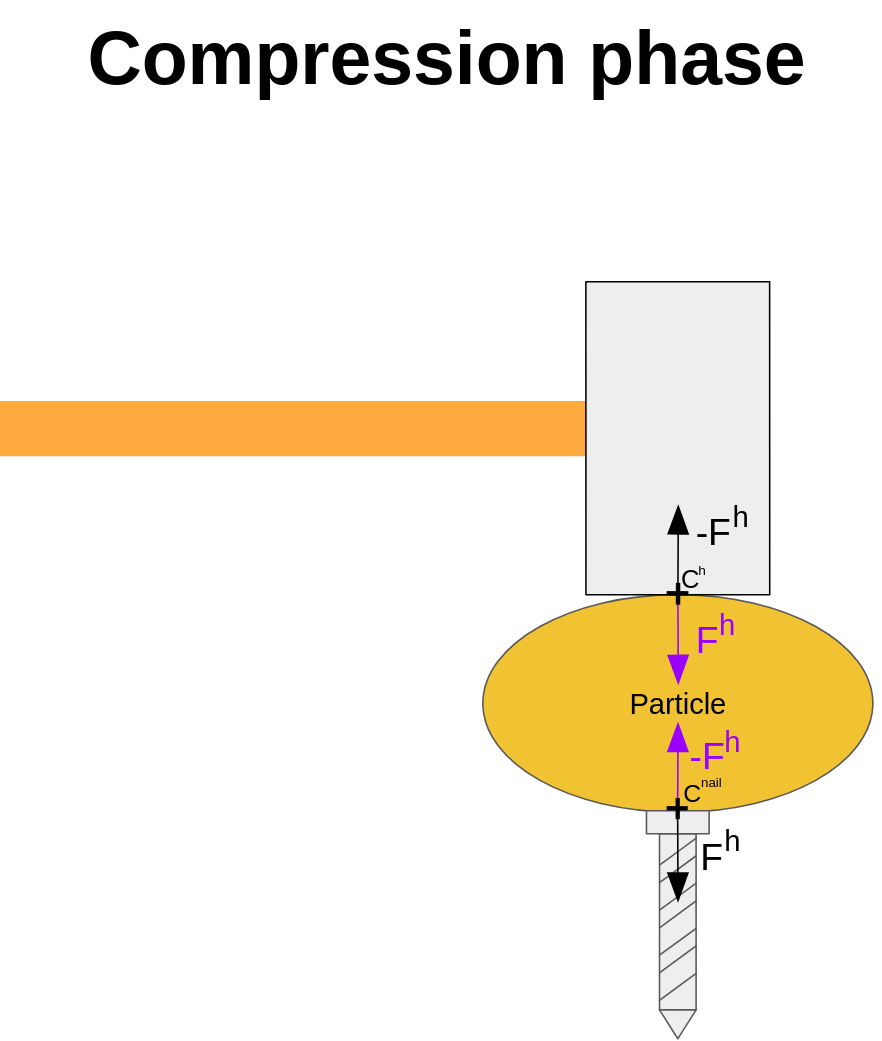
\includegraphics[width=0.5\linewidth]{Compression phase.png}
%     \caption{Compression phase}
%     \label{COMPRESSION PHASE}
%     \centering
%     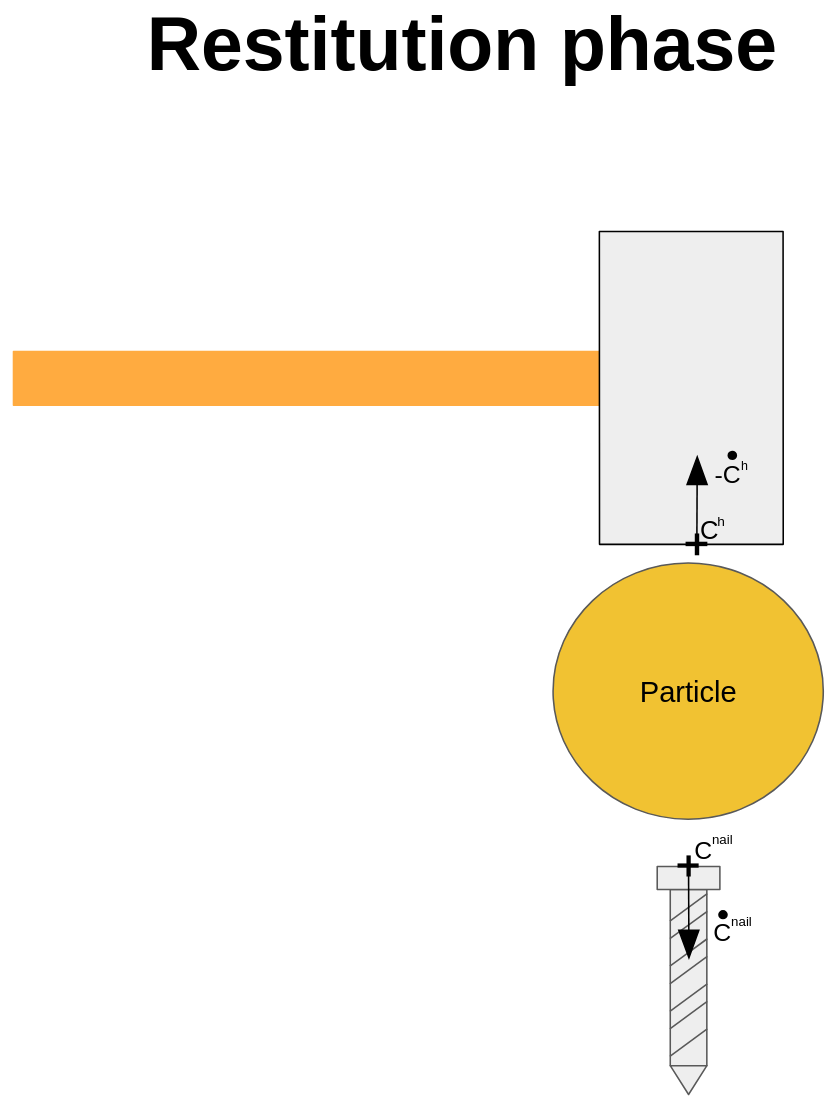
\includegraphics[width=0.5\linewidth]{Restitution phase.png}
%     \caption{Restitution phase}
%     \label{RESTITUTION PHASE}
% \end{figure*}

% \begin{figure*}
%     \vspace*{-2.5cm}
%     \centering
%     \includesvg[width=0.9\linewidth]{All_phases.svg}
%     \caption{Particle impact phases}
%     \label{Particle impact phases}
% \end{figure*}
\subsection{Direct impact model}
\begin{figure}
    \centering
    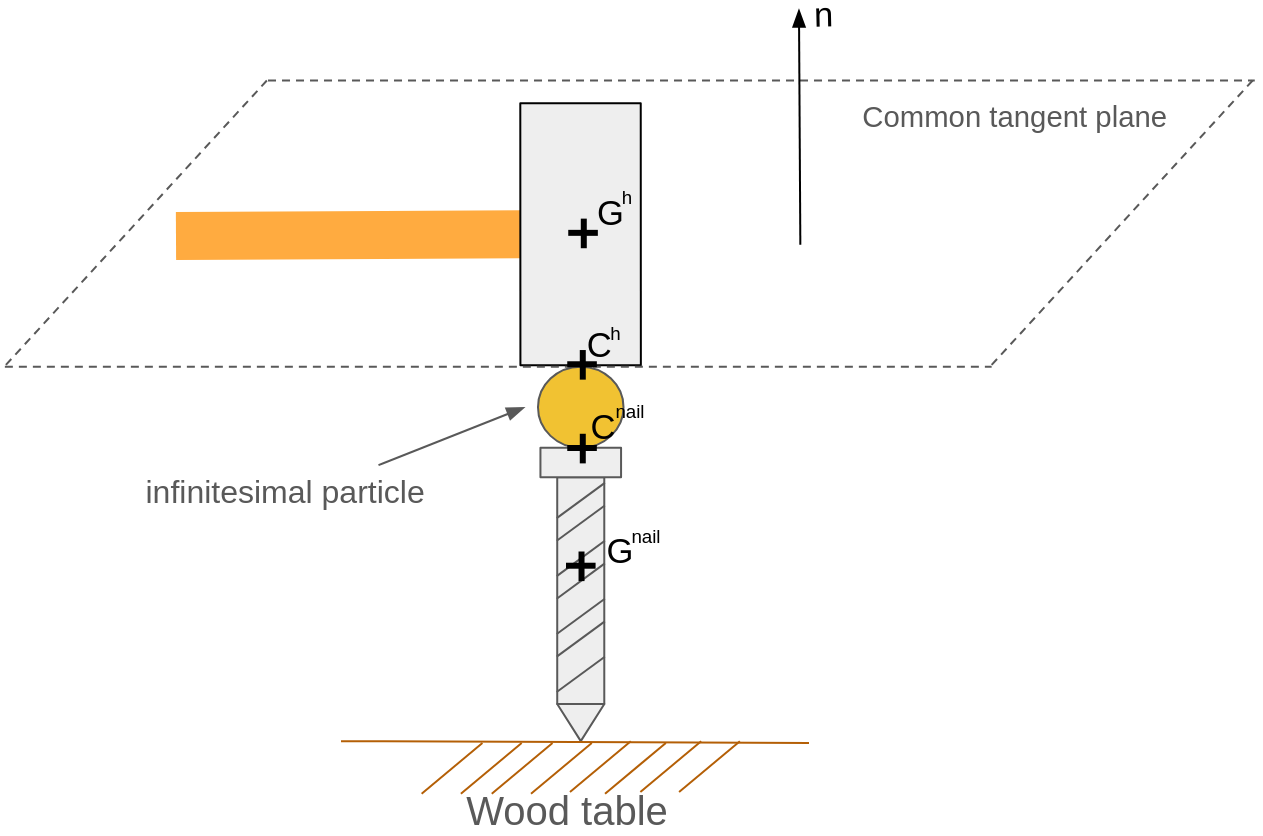
\includegraphics[width=0.84\linewidth]{Schematic of the problem.png}
    \caption{Schematic of the collision between the hammer tip and the nail modeled as a particle impact.}
    \label{SCHEMATIC OF THE PROBLEM}
\end{figure}
\noindent
Let $\mathbf{x}_{\nu}(t)$ and $\mathbf{c}^{nail}(t) \in \mathbb{R}^3$ be the contact points of the hammer tip and the nail expressed in the world frame $w$, respectively, as illustrated by Fig.~\ref{SCHEMATIC OF THE PROBLEM}. 
At the instant of contact $t_c$, these points collide and thus share the same coordinates (neglecting the radius of the particle, see Fig.~\ref{SCHEMATIC OF THE PROBLEM}):
\begin{equation}
    \mathbf{x}_{\nu}(t_c) = \mathbf{c}^{nail}(t_c)
\end{equation}
% The nail is stationary before impact, i.e. from the initial time $t_i$ to the instant of contact $t_c$ its velocity is $\mathbf{0}$:
% \begin{equation}
%     \mathbf{\dot c}^{nail}(t) = \mathbf{0} \ \ \ \  \forall t \in [t_i, t_c]
% \end{equation}
The velocity and acceleration of the hammer tip are given by the trajectory that will be introduced in Section \ref{Hammer tip velocity and acceleration}. 
% When the colliding bodies first interact, the contact points $C$ and $C'$ have an initial relative velocity $v_0$:
% \begin{equation}
%     \mathbf{v_{0}} = \mathbf{V}_C(0) - \mathbf{V}_{C'}(0)
% \end{equation}
% which has a component $\mathbf{v_0} \cdot \mathbf{n}$ normal to the common tangent plane.

A direct impact is an impact that occurs when the relative approaching velocity of the colliding bodies is parallel to $\mathbf{n}$ \cite{STRONGE}. 
Our goal with the hammering problem is to achieve a direct impact. 
We will assume that it is indeed the case, thus there will be no tangential sliding during impact.

\subsection{Projected momentum of the hammer tip}
\noindent
To quantify an impact, we define the normal impulse $i \in \mathbb{R}$ given by the hammer tip to the nail over an infinitesimal duration $\delta t$ to be: 
\begin{equation}
    i \triangleq \int_{t_c}^{t_c + \delta t} 
    %m \frac{d}{d\tau} \mathbf{\dot x_\nu^T n} \ d\tau
    \mathbf{n^T} \mathbf{F}^hdt
\label{impulse}
\end{equation}
To maximize the impact, we want to maximize the impulse given by (\ref{impulse}) which is equivalent to maximizing the projected momentum $P(t) \in \mathbb{R}$ of the hammer tip along the normal $\mathbf{n}$ \cite{SinglePointParticle} defined as:
\begin{equation}
    P(t) \triangleq m_{e,\mathbf{n}}(\mathbf{q})  \mathbf{\dot x_{\nu}^T} \mathbf{n} 
\label{Momentum end effector}
\end{equation}
This is because: 
\begin{equation}
    i = \Delta P = P(t_c + \delta t) - P(t_c)
\end{equation}
For a fixed given target normal velocity $\mathbf{\dot x_\nu^T n}$, we see that in order to maximize the projected momentum of the hammer tip, we have to maximize the EMR. This procedure is explained in Section \ref{Optimization of the effective mass using QP}.

% \subsection{Particle impact}
% \noindent
% When the hammer tip collides with the particle, the particle will deform during the compression phase and store elastic strain energy. That energy will be released during the restitution phase and drive the hammer tip upwards and the nail downwards (see Fig.~\ref{Particle impact phases}). From that, let us establish a mathematical model to assess the velocities of the robot and of the nail after impact. 
% Let us define the effective mass of the collision $m \in \mathbb{R^+}$:
% \begin{equation}
%     m \triangleq \frac{m_{e,\mathbf{n}} m_n}{m_{e,\mathbf{n}} + m_n}
% \label{Effective mass of the collision}
% \end{equation}
% where $m_n$ is the mass of the nail which is very light compared to the EMR. Because of that, we have $m_n << m_{e,\mathbf{n}}$ and (\ref{Effective mass of the collision}) becomes:
% \begin{equation}
%     m = m_n
% \label{approx effective mass of the collision}
% \end{equation}
% % Let $\mathbf{v_-} \in \mathbb{R}^3$ be the desired pre-impact velocity vector of the hammer tip. 
% For ease of notation, let us introduce: 
% \begin{equation}
%     \mathbf{\dot x}_{\nu}^{t_c} \triangleq \mathbf{\dot x}_{\nu}(t_c)
% \end{equation}
% From the particle impact model of Stronge \cite{STRONGE}, 
% the post-impact velocity of the hammer tip $\mathbf{\dot x}_{\nu}^{+}$ 
% %$\mathbf{v_+} \in \mathbb{R}^3$ 
% is given by:
% %\textcolor{red}{\textbf{How to define $t_f$ ?}}
% \begin{equation}
% \begin{split}
%     \mathbf{\dot x}_{\nu}^{+} 
%     %&= \mathbf{\dot C}^{h}(t_c) - \frac{m}{m_{e, \mathbf{n}}}(1+e_*) \mathbf{\dot C}^{h}(t_c)\\
%                  &= \left[ 1-\frac{m}{m_{e, \mathbf{n}}} (1+e_*)\right] \mathbf{\dot x}_{\nu}^{t_c} 
%                  % \\ & = \alpha \mathbf{\dot x}_{\nu}^{t_c} 
%                  %\ \ \ \ \forall t \in [t_c, t_f]
% \label{Post-impact velocity of the hammer tip}
% \end{split}
% \end{equation}
% % where the scalar $\alpha$ is introduced for ease of notation:
% % \begin{equation}
% %     \alpha = 1-\frac{m}{m_{e, \mathbf{n}}} (1+e_*)
% % \end{equation}
% From the same model, the velocity of the nail after impact $\mathbf{\dot c}^{nail, +}$ 
% %$\mathbf{v_+^{nail}} \in \mathbb{R}^3$ 
% is:
% \begin{equation}
% \begin{split}
%     \mathbf{\dot c}^{nail, +} &= \frac{m}{m_n} (1+e_*) \mathbf{\dot x}_{\nu}^{t_c} 
%                               = (1+e_*) \mathbf{\dot x}_{\nu}^{t_c} 
%                               %\ \ \ \ \forall t > t_c
% \end{split}
% \label{Post-impact velocity of the nail}
% \end{equation}
% by the hypothesis given by (\ref{approx effective mass of the collision}). \\
% Equation (\ref{Post-impact velocity of the hammer tip}) shows that the hammer tip will be subject to a rebounce after impact and (\ref{Post-impact velocity of the nail}) shows that the velocity of the nail after getting hit depends on the pre-impact velocity of the hammer tip, which makes sense intuitively. The rebounce might destabilize the robot, but this problem is out of the scope of this paper.


% \subsection{Hit effectiveness with an energy approach}
% \textcolor{red}{\textbf{REFORMULATE OR REWRITE THIS PART ? IS IT THE DIFFERENCE IN THE NAIL KINETIC ENERGY OF THE NAIL OR THE HAMMER KINETIC ENERGY? DO WE EVEN KEEP THIS PART ?}} \\\\
% % When the hammer hits the nail, if the nail does not move then there is a rebounce. Otherwise, the hammer will follow the nail through the wood (which means we could consider the \{hammer+nail\} system as a single object moving with some velocity $v$) and continuously give the nail kinetic energy to make it penetrate the wood until there is no more kinetic energy.
% % The rebounce is related to the coefficient of restitution. \\
% %\subsection{Constant force} 
% Let $W \in \mathbb{R^+}$ be the net work done on the nail by the hammer tip.
% If the hammer hits the nail with enough force, the impulsive force generated by the hammer tip will be constant and equal to the force needed to overcome stiction. The duration of the motion of the nail penetrating the wood will be longer, thus the nail would penetrate more wood \cite{CITATION?}.
% Let us say that we need at least an energy $E_{crit}$ to displace the nail \cite{CITATION?}. Anything below that threshold would result in no displacement of the nail (or so vanishingly small it can be considered to be 0). Let $K_-$ be the kinetic energy of the hammer tip just before hitting the nail. Then:
% \begin{itemize}
%     \item If $K_- < E_{crit}$ then $W = 0$ because the displacement $\delta d = 0$, we can set $e_*=1$ or to a scalar close to 1,
%     \item If $K_- \ge E_{crit}$ then $W \ne 0$, $\mathbf{n^T} \mathbf{F}^h \ne 0$ and $\delta d \ne 0$, we can set $e_*=0$ or to a scalar close to $0$.
% \end{itemize}
% To estimate the hit effectiveness, we use the work-energy theorem, which states that the net work done on the nail equals the change in its kinetic energy: 
% \begin{equation}
%     W = \Delta K
% \end{equation}
% where $\Delta K$ is the difference of the hammer tip's normal kinetic energy \textcolor{red}{\textbf{or is it the nail's ?}}:
% \begin{equation}
%     \Delta K =  K_+ - K_-
% \end{equation}
% with:
% \begin{equation}
%     K_+ = \frac{1}{2}m_{e,\mathbf{n}}(\mathbf{v_+^T n})^2
% \end{equation}
% \begin{equation}
%     K_- = \frac{1}{2}m_{e,\mathbf{n}}(\mathbf{n^T }\mathbf{\dot x}_{\nu}^{t_c})^2
% \end{equation}
% Thanks to that, we can compute the penetration $\delta d \in \mathbb{R^+}$ of the nail into the wood. 
% % The hammer tip is colliding with the nail with some normal kinetic energy $K_- \in \mathbb{R}^+$: 
% % \begin{equation}
% %     K_- = \frac{1}{2}m_{e,\mathbf{n}}(\mathbf{v_-^T n})^2
% % \end{equation}
% This kinetic energy is transferred to the nail and makes it moves through the wood. The amount of penetration is given by:
% \begin{equation}
% \begin{split}
%     \delta d &= \frac{1}{2\mathbf{n^T} \mathbf{F}^h} m_{e,\mathbf{n}}\left( (\mathbf{v_+^T n})^2 - (\mathbf{n^T}\mathbf{\dot x}_{\nu}^{t_c})^2 \right)  \\
%             & = \frac{\alpha^2 -1}{2 \mathbf{n^T} \mathbf{F}^h} m_{e,\mathbf{n}} (\mathbf{n^T} \mathbf{\dot x}_{\nu}^{t_c})^2 \\
% \end{split}
% \end{equation}
% where $\mathbf{F}^h$ is the force applied to the nail by the hammer which can be obtained thanks to Coulomb's friction law \textcolor{red}{\textbf{GIVE EXPRESSION OF $\mathbf{F}^h$ ?}}. However, as stated in Section \ref{Energy-based model}, we have to remember that we do not take into account the other types of energy, thus this model is only an approximation of the real wood penetration.
% \subsection{Maintaining the Integrity of the Specifications}

% The IEEEtran class file is used to format your paper and style the text. All margins, 
% column widths, line spaces, and text fonts are prescribed; please do not 
% alter them. You may note peculiarities. For example, the head margin
% measures proportionately more than is customary. This measurement 
% and others are deliberate, using specifications that anticipate your paper 
% as one part of the entire proceedings, and not as an independent document. 
% Please do not revise any of the current designations.

\section{Maximization of the effective mass of the robot using QP}
\label{Optimization of the effective mass using QP}
\noindent
The following section presents our QP formulation, in which EMR maximization is included as a weighted objective.
\subsection{Tasks}
\noindent
Let us first introduce what we call a ``task". A task is an objective that the robot has to accomplish, for instance maintaining a posture or moving its end-effector to a desired position.
To realize a task, we compute a desired configuration acceleration $\mathbf{\ddot q_d}$, then we track how well the robot realizes this task using a cost function expressed as a function of the actual configuration acceleration $\mathbf{\ddot q}$.
\subsection{Formulation of the problem to solve}
\label{QP formulation of EMMT}
\noindent
For this part, our decision variable is the configuration acceleration $\mathbf{\ddot q}$. In order to make it appear at the expression of the effective mass, we differentiate the EMR twice with respect to time:
\begin{equation}
        \dot m_{e,\mathbf{n}} (\mathbf{q}, \mathbf{\dot q}) = \frac{d m_{e,\mathbf{n}}}  {d\mathbf{q} } \frac{d\mathbf{q}}{dt} 
    = \nabla m_{e,\mathbf{n}}^\mathbf{T}(\mathbf{q})  \mathbf{\dot q}
\label{time derivative of the effective mass}
\end{equation}
\begin{equation}
            \ddot m_{e,\mathbf{n}} (\mathbf{q}, \mathbf{\dot q}, \mathbf{\ddot q}) = \frac{d}{dt} \left\{ \nabla m_{e,\mathbf{n}}^\mathbf{T}(\mathbf{q) } \right\} \mathbf{\dot q} + \nabla m_{e,\mathbf{n}}^\mathbf{T}(\mathbf{q) } \mathbf{\ddot q}
\label{double time derivative of m}
\end{equation}
From (\ref{double time derivative of m}), we can reconstruct $m_{e,\mathbf{n}}$ by discrete time integration. Let $\Delta t$ be the timestep of the controller, then we have:
\begin{equation}
    %m_{e,\mathbf{n}}(\mathbf{q}) = \int_{t_i} ^{t_f} \int_{t_i}^{t_f} \ddot m_{e,\mathbf{n}}(\mathbf{q}(t), \mathbf{\dot q}(t), \mathbf{\ddot q}(t)) dt
    m_{e,\mathbf{n}}(\mathbf{q}(t + \Delta t)) =  m_{e,\mathbf{n}} + \dot m_{e,\mathbf{n}}\Delta t+ \ddot m_{e,\mathbf{n}}\frac{\Delta t^2}{2}
\end{equation}
Taking $\arg \max_{\mathbf{\ddot q}}$ on both sides, the first two terms of the right hand side of the equation are discarded because they do not depend on $\mathbf{\ddot q}$, then  by (\ref{effective mass}) and (\ref{time derivative of the effective mass}) we have:
\begin{equation}
    \arg \max_{\mathbf{\ddot q}}m_{e,\mathbf{n}}(\mathbf{q}(t + \Delta t)) =  \arg \max_{\mathbf{\ddot q}} \ddot m_{e,\mathbf{n}}
\end{equation}
%where $t_i$ is the starting time and $t_f$ is the final time, $t_f  > t_i$.
Thus, in order to maximize $m_{e,\mathbf{n}}$ with respect to $\mathbf{\ddot q}$, we have to maximize $\ddot m_{e,\mathbf{n}}$. Therefore, we want to solve:
\begin{equation}
    \arg \max_\mathbf{\ddot q} \left\{ \frac{d}{dt} \left\{ \nabla m_{e,\mathbf{n}}^\mathbf{T}(\mathbf{q}) \right\} \mathbf{\dot q} + \nabla m_{e,\mathbf{n}}^\mathbf{T}(\mathbf{q) } \mathbf{\ddot q} \right\}
\end{equation}
Again, because our decision variable is $\mathbf{\ddot q}$, we can drop the first term which does not depend on the configuration acceleration $\mathbf{\ddot q}$ and we are left with:
\begin{equation}
    \arg \max_\mathbf{\ddot q} \nabla m_{e,\mathbf{n}}^\mathbf{T}(\mathbf{q})  \mathbf{\ddot q}
\label{max problem}
\end{equation}
which avoids differentiating the gradient with respect to time. \\
As the QP is defined as a minimization problem, we can rewrite (\ref{max problem}) as such in the following way:
% As the QP in the mc\_rtc framework uses a minimization problem, we can rewrite  to a minimization problem in the following way:
\begin{equation}
    \arg \min_\mathbf{\ddot q} -\nabla m_{e,\mathbf{n}}^\mathbf{T}(\mathbf{q})  \mathbf{\ddot q}
\label{minimization problem}
\end{equation}
Let us call this objective function the Effective Mass Maximization Task (EMMT). 
The goal of this task is to increase as much as possible the EMR at the next iteration of the controller. 
However, we cannot assert that the result will be a global maximum because our problem is not necessarily convex.
Note that this scheme shares some similarities with the work of Wang and Kheddar~\cite{wangImpactFriendlyRobustControl2019}, where the momentum of the impact is maximized using a QP. 
However, in that work the effective mass was considered constant and its maximization was not part of the objectives 
%If we want to try to find a global maximum, we might need to use other methods, although these ones are generally much slower. 
\subsection{Linear QP constraints to be respected}
\label{QP constraints}
\noindent
Our linear constraints for the QP solver are described as i) joint limits, ii) joint velocity limits, and iii) joint torque limits.
% \begin{equation}
%     \mathbf{q_{LB}} \preceq \mathbf{q} \preceq \mathbf{q_{UB}}
% \label{Joint limits}
% \end{equation}
% \begin{equation}
%     \mathbf{\dot q_{LB}} \preceq \mathbf{\dot q} \preceq \mathbf{\dot q_{UB}}
% \label{Joint velocity limits}
% \end{equation}
% % \begin{equation}
% %     \mathbf{\ddot q_{LB}} \preceq \mathbf{\ddot q} \preceq \mathbf{\ddot q_{UB}}
% % \label{Joint acceleration limits}
% % \end{equation}
% \begin{equation}
%     \bm \tau_{\mathbf{LB}} \preceq \bm \tau \preceq \bm \tau_{\mathbf{UB}}
% \label{Torque limits}
% \end{equation}
% \begin{equation}
%     \bm \kappa_{\xi} = \left(d_i, d_s, \xi_{offset}\right)^\mathbf{T}
% \label{Dynamic constraints}
% \end{equation}
% where the subscripts $\mathbf{LB}$ and $\mathbf{UB}$ mean "Lower Bound" and "Upper Bound", respectively, $\bm \tau \in \mathbb{R}^n$ is the actual vector of joint torques and the $\preceq$ operator is the term-by-term comparison operator between two vectors of $\mathbb{R}^n$.
% For the dynamic constraints (\ref{Dynamic constraints}), $d_i$ is the interaction distance, $d_s$ is the security distance and $\xi_{offset}$ is a fixed offset, 
These are all defined in the sense of Vaillant et al. ~\cite{vaillantMulticontactVerticalLadder2016}.


\subsection{Implementation of the EMMT}
\noindent
The posture task is a task where the robot has to maintain a given configuration $\mathbf{q}$. Cisneros et al. \cite{cisnerosRobustHumanoidControl2018} gives a deeper look into it. 
From the complete cost function in our QP formulation:
\begin{equation}
    \arg \min_{\mathbf{\ddot q}} \frac{1}{2}W_{p}\| \mathbf{\ddot q} + \mathbf{b}\|^2 - W_m \nabla m_{e,\mathbf{n}}^
\mathbf{T}(\mathbf{q}) \mathbf{\ddot q} + A(\mathbf{\ddot q})
\label{Global QP}
\end{equation}
the first term represents the posture task, the second term is the EMMT and $A(\mathbf{\ddot q}) \in \mathbb{R}$ is the cost function associated to the other possible tasks that the robot has to realize (for instance, a trajectory task). $W_p$, $W_m \in \mathbb{R^+}$  are the relative weights associated to the posture task and the EMMT, respectively, and $\mathbf{b} \in \mathbb{R}^n$ is a PD controller written as: 
\begin{equation}
    \mathbf{b} = K_p(\mathbf{q - q_d}) + K_d(\mathbf{\dot q - \dot q_d}) - \mathbf{\ddot  q_d}
\label{PD controller}
\end{equation}
where $K_p$ and $K_d$ are the proportional (stiffness) and derivative (damping) gains of the posture task, respectively, $\mathbf{q_d}$, $\mathbf{\dot q_d}$, $\mathbf{\ddot q_d} \in \mathbb{R}^n$ are the desired configuration, desired configuration velocity and desired configuration acceleration, respectively.\\
The relationship between $K_p$ and $K_d$ is given by:
\begin{equation}
    K_d = 2\sqrt{K_p}
\label{Kp Kd relationship}
\end{equation}
To implement our EMMT task, we will modify (\ref{Global QP}) in the following way:
\begin{equation}
     \arg \min_{\mathbf{\ddot q}} \frac{1}{2}W_p \|\mathbf{\ddot q +b} - \frac{W_m}{W_p} \nabla m_{e, \mathbf{n}}(\mathbf{q}) \|^2 + A(\mathbf{\ddot q})
\label{Trick}
\end{equation}
subject to the constraints presented in Section~\ref{QP constraints}. 
This guarantees the problem is strictly convex and can be solved with least square solvers.
% (\ref{Joint limits}), 
% (\ref{Joint velocity limits}), 
% % (\ref{Joint acceleration limits}), 
% (\ref{Torque limits}) 
% and (\ref{Dynamic constraints}). 

This approach allows us to maximize the EMR online instead of optimizing offline.
More importantly, it would require high tracking gains to strictly follow the planned kinematic trajectory which increases the risks of robot damage. 
% Using an offline method implies knowing the pose of the hitting target in advance every time, and this would not work if we were to change the pose of the nail.
% Furthermore, the feasibility of reaching the desired posture is also an issue with an offline method, as it is not trivial to suggest an appropriate posture due to the high redundancy of the robot.

\section{Trajectory of the end-effector}
\label{Trajectory of the end-effector}
\noindent
In this section, we present how the end-effector of the robot reaches the nail with a given velocity. 

\subsection{B-Spline trajectory task}
\label{BSplineTrajectoryTask}
\noindent
The primary task of the end-effector is to reach the nail with a given velocity. To do that, we use a continuous Bézier curve as our trajectory, which is a specific case of a B-Spline. Let us call that task the B-Spline trajectory task (BSTT).

A $(N+1)$-points Bézier curve $\bm \Gamma: \mathbb{R} \to \mathbb{R}^3$, or $N$-th order Bézier curve, is defined as: 
\begin{equation}
    \bm \Gamma(t) \triangleq \sum_{k=0}^{N} B^N_k \left( \frac{t-t_{i}}{T} \right) \mathbf{p}_k \ \ \ \ \forall t \in [t_i, t_c]
\label{Bézier curve}
\end{equation}
where $[t_{i}, t_{c}]$ is the time interval on which $\bm \Gamma$ is defined, $t_{c} > t_{i}$, $\mathbf{p}_k \in \mathbb{R}^3$ is the constant $k$-th control point of the curve, $T = t_{c} - t_{i}$ and $B^N_k$ is a Bernstein polynomial that acts as a weight \cite{ComputerGraphics}, such that: 
\begin{equation}
        B^N_k \left( \frac{t-t_{i}}{T} \right) \triangleq \binom{N}{k} \left( \frac{t-t_{i}}{T} \right)^k \left(1-\frac{t-t_{i}}{T}\right)^{N-k}
    \label{bernstein polynomial}
\end{equation}
The first control point of the curve, $\mathbf{p_0}$, is the 3D initial position of the hammer tip, $\mathbf{x}_{\nu}^{t_i} \in \mathbb{R}^3$ (the subscript ``\textit{i}" stands for ``\textit{initial}"), and the last control point, $\mathbf{p_N}$, is the 3D position of the nail $\mathbf{c}^{nail} \in \mathbb{R}^3$, both with respect to the fixed world frame. Thus:
\begin{equation}
    \mathbf{p_0} = \mathbf{x}_{\nu}^{t_i}
\end{equation}
\begin{equation}
    \mathbf{p_N} = \mathbf{c}^{nail} 
\end{equation}
These points have the property of acting as waypoints for the trajectory, which is not the case for the potential in-between points.
%\textcolor{red}{\textbf{COST FUNCTION OF THE BSPLINE TASK ?}}\\
% Let $\bm \epsilon_{\mathbf{x}}(t) = \mathbf{x_\nu}(t) - \bm \Gamma (t) \in \mathbb{R}^3$ be the position error vector of the end-effector between its current position and its desired position given by the Bézier curve at time $t$. The cost function of the BSTT is:
% \begin{equation}
%     C_{BSTT}(\mathbf{\ddot q}) = \|K_{p, B} \bm \epsilon_{\mathbf{x}} + K_{d, B} \bm{ \dot \epsilon_{\mathbf{x}}} - \mathbf{\dot J_\nu \dot q} - \mathbf{J_\nu \ddot q}\|^2
% \end{equation}
% where $K_{p, B}$ and $K_{d, B} \in \mathbb{R^+}$ are respectively the stiffness and damping coefficient of the BSTT.
\subsection{Curve constraints}
\label{Curve constraints}
\noindent
To make the end-effector reach the desired velocity when hitting the nail, we constrain the curve by adding four control points $\mathbf{p_{c_1}}$, $\mathbf{p_{c_2}}$, $\mathbf{p_{c_{N-1}}}$ and $\mathbf{p_{c_{N-2}}} \in \mathbb{R}^3$ . These added points count towards the degree of the curve. The expression of the added points is given by \cite{NDCURVESLIB}:
\begin{equation}
    \mathbf{p_{c_1}} = \mathbf{p_0} + \frac{T}{N} \bm {\kappa}_{\mathbf{\dot x}_{\nu}^{t_i}}
\end{equation}
\begin{equation}
    \mathbf{p_{c_2}} = 2\mathbf{p_{c_1}} - \mathbf{p_0} + \frac{T^2}{\left(N-1 \right) \left(N-2 \right)} \bm {\kappa}_{\mathbf{\ddot x}_{\nu}^{t_i}}
\end{equation}
which are added just after $\mathbf{p_0}$, where $\bm {\kappa}_{\mathbf{\dot x}_{\nu}^{t_i}} \in \mathbb{R}^3$ are the initial linear velocity constraints and $\bm {\kappa}_{\mathbf{\ddot x}_{\nu}^{t_i}} \in \mathbb{R}^3$ are the initial linear acceleration constraints.
Also:
\begin{equation}
    \mathbf{p_{c_{N-1}}} = \mathbf{p_N} - \frac{T}{N -1} \bm {\kappa}_{\mathbf{\dot x}_{\nu}^{t_c}}
\end{equation}
\begin{equation}
    \mathbf{p_{c_{N-2}}} = 2\mathbf{p_{c_{N-1}}} - \mathbf{p_N} + \frac{T^2}{\left(N-1 \right) \left(N-2 \right)} \bm {\kappa}_{\mathbf{\ddot x}_{\nu}^{t_c}}
\end{equation}
where $\bm {\kappa}_{\mathbf{\dot x}_{\nu}^{t_c}} \in \mathbb{R}^3$ are the linear final velocity constraints and $\bm {\kappa}_{\mathbf{\ddot x}_{\nu}^{t_c}} \in \mathbb{R}^3$ are the final linear acceleration constraints.
Thus, if we add the curve constraints, we will have six control points in total, hence a $5^{th}$ order Bézier curve.

\subsection{Hammer tip velocity and acceleration}
\label{Hammer tip velocity and acceleration}
\noindent
The desired velocity $\mathbf{\dot x}_{\nu, d}$ and acceleration $\mathbf{\ddot x}_{\nu, d}$ of the hammer tip from the initial instant $t_i$ to the instant of contact $t_c$ expressed with respect to the world frame $w$ are given by the first and second time derivative of (\ref{Bézier curve}), respectively:
\begin{equation}
    \mathbf{\dot x}_{\nu, d}(t) = \bm {\dot \Gamma}(t) \ \ \ \ \forall t \in [t_i, t_c]
\end{equation}
\begin{equation}
    \mathbf{\ddot x}_{\nu, d}(t) = \bm {\ddot \Gamma}(t) \ \ \ \ \forall t \in [t_i, t_c]
\end{equation}
Both the velocity and acceleration of the hammer tip are affected by the curve constraints (more precisely, the added control points) defined in Section \ref{Curve constraints}. 

Let $\epsilon_{\mathbf{x}_\nu} = \mathbf{x}_\nu - \mathbf{x}_{\nu, d}$ where $\mathbf{x}_{\nu, d}$ is the desired end-effector position given by $\bm \Gamma$. The cost function of the BSTT, $A_{B}(\mathbf{\ddot q})$, is:
\begin{small}
    \begin{equation}
        A_{B}(\mathbf{\ddot q}) = W_{B}\| K_{p, B} \bm \epsilon_{\mathbf{x}_\nu}+ K_{d, B} \bm {\dot \epsilon_{\mathbf{x}_\nu}} + \mathbf{\ddot x}_{\nu, d} - \mathbf{\dot J_\nu \dot q} - \mathbf{J_\nu \ddot q} \|^2
    \end{equation}
\end{small}
\noindent
where $W_B \in \mathbb{R}^+$ is the relative weight associated to the BSTT and $K_{p, B}$, $K_{d, B} \in \mathbb{R}^+$ are its stiffness and damping, respectively.

\subsection{Orientation of the hammer tip}
\label{VectorOrientationTask}
\noindent
In addition to reaching the nail, we have to orient the hammer tip such that the impact with the nail axis is \textit{collinear}. Let $\mathbf{G}^{h}$, $\mathbf{G}^{nail} \in \mathbb{R}^3$ be the center of mass of the hammer tip and the center of mass of the nail, respectively. 
A collinear impact is an impact where $\mathbf{G}^h$, $\mathbf{G}^{nail}$ and the contact points $\mathbf{x}_\nu$ and $\mathbf{c}^{nail}$ are aligned \cite{STRONGE}, see Fig.~\ref{SCHEMATIC OF THE PROBLEM}. 
We constraint two rotation DOFs: the roll and the pitch of the hammer tip, and we let the yaw be free. 
Indeed, we want to align three vectors: the vector normal to the contact surface of the hammer tip which we will call $\mathbf{n}^h \in \mathbb{R}^3$ (expressed in the hammer tip frame), and the normal vector at the top of the nail. 
% The latter is already done by the path to the nail. 
% Tilt alignment: go from $(\alpha_1, \beta_1)$ to $(\alpha_2, \beta_2)$. The error between the vectors can be the cosine of the angle between them (aligned vectors in the same direction have a cosine equal to 1 or substract the vectors to get the direction of the error).

Let $\mathbf{R}_{w \to h}$ be the rotation matrix describing the rotation of the hammer tip from the world frame, $\bm \epsilon = \mathbf{n}^h - \mathbf{n}$ the error vector between the desired vector ($\mathbf{n}$) and the actual vector ($\mathbf{n}^h$), $\mathbf{\dot x}_{\omega} \in \mathbb{R}^{3}$ the angular velocity vector of the hammer tip in the world frame given by:
% \textcolor{red}{\textbf{what is that}}
\begin{equation}
    \mathbf{\dot x}_{\omega} = -\mathbf{R}_{w \to h}  \left[\mathbf{n}^h \right]_{\times} \mathbf{J_\omega \dot q}
\label{hammer tip angular velocity}
\end{equation}
where $\left[ \cdot \right]_{\times}: \mathbb{R}^3 \to \mathbb{R}^{3 \times 3}$ is the skew-symmetric operator defined, for all $\mathbf{a} =(a_x, a_y, a_z)^\mathbf{T} \in \mathbb{R}^3$, as:
\begin{equation}
\left[ \mathbf{a} \right]_{\times} = 
\begin{bmatrix}
    0 & - a_z & a_y \\
    a_z & 0 & -a_x \\
    -a_y &  a_x & 0
\end{bmatrix}
\end{equation}
The time derivative of (\ref{hammer tip angular velocity}) is:
{\small
\begin{equation}
    \mathbf{\ddot x}_{\omega} = -\mathbf{\dot R}_{w \to h}\left[\mathbf{n}^h \right]_{\times} \mathbf{J_\omega \dot q} - \mathbf{R}_{w \to h}\left[\mathbf{n}^h \right]_{\times}\left( \mathbf{J_{\omega} \ddot q + \dot J_{\omega} \dot q} \right)
\end{equation}
}
% From the starting orientation of the hammer, the rotation needed $\mathbf{R}_{tot} \in SO(3)$ to have a collinear impact is:
% \begin{equation}
%     \mathbf{R}_{tot} = \mathbf{R}_{0} \mathbf{R}_{w \to nail}^{\mathbf{T}}
% \end{equation}
% where $\mathbf{R}_0 \in SO(3)$ is an "offset" rotation to properly "align the axis, i.e. the normal of the hammer, the normal of the nail and the vector between the hammer tip and the nail" \textcolor{red}{REFORMULATE THAT}. \\
\noindent
Let us call this task the Vector Orientation Task (VOT).
The cost function of this task is:
\begin{equation}
     A_{VOT}(\mathbf{\ddot q}) = W_{VOT}\| K_{p, VOT} \bm \epsilon + K_{d,VOT} \bm {\dot \epsilon}- \mathbf{\ddot x}_{\omega}(\mathbf{\ddot q}) \|^2 
\end{equation}
where $W_{VOT}$ is the relative weight associated to the VOT and $K_{p, VOT}$, $K_{d, VOT} \in \mathbb{R}^+$ are its stiffness and damping, respectively. 
\begin{figure}
    \centering
    \includesvg[width=0.7\linewidth]{EMMT 1_1}
    \caption{Time evolution of the EMR with only a posture task active.}
    \label{Time evolution of the effective mass of the robot 1}
\end{figure}
\begin{figure}
    \centering
    \includesvg[width=0.7\linewidth]{Projected_momentum}
    \caption{Time evolution of the projected momentum along the normal $\mathbf{n}$.}
    \label{Time evolution of the momentum projected along the normal n}
\end{figure}
\section{Simulations with the robot}
\label{Simulations}
\begin{figure*}
    % \vspace*{-2.3cm}
    \centering
    \includesvg[width=0.68\linewidth]{Velocities}
    \caption{Velocity tracking of the hammer tip for different $K_{p, VOT}$ values.}
    \label{Velocity tracking of the hammer tip}
\end{figure*}
% \begin{figure}
%     % \vspace*{-2.3cm}
%     \centering
%     \includesvg[width=0.8\linewidth]{VelocityA}
%     \caption{Velocity tracking of the hammer tip for $K_{p, VOT} = 1000$.}
%     \label{VelocityA tracking of the hammer tip}
% \end{figure}
% \begin{figure}
%     % \vspace*{-2.3cm}
%     \centering
%     \includesvg[width=0.8\linewidth]{VelocityB}
%     \caption{Velocity tracking of the hammer tip for $K_{p, VOT} = 250$.}
%     \label{VelocityB tracking of the hammer tip}
% \end{figure}
\noindent
In this section, we present the simulations made on our humanoid robot HRP-5P. The setting is a fixed hammer attached to one of the robots' grippers (the left one in our case), a fully known position and orientation of the nail and a prefixed desired hitting velocity of the hammer tip on the nail.  
Simulations were done using mc\_mujoco and mc\_rtc \cite{singhMcmujocoSimulatingArticulated2022} with its QP solver in torque control mode, and a timestep $\Delta t = 0.002$s 
% and dynamic constraints set to $\bm \kappa_{\xi} = (0.1, 0.01, 0.5)^\mathbf{T}$
. 
The floating base of the robot is fixed as keeping balance after the impact is out of the scope of this paper. 
The hammer used weighs 0.792 kg, has a length of 328 mm and its contact surface is circular with radius 15.5 mm. 
The nail is fixed and ``floating" in the environment to avoid earlier or post-impact collisions with an object (such as a table), it has a length of 88.03 mm and its head has a radius of 6.95 mm. 
The tasks at play are the EMMT within the posture task defined in Section \ref{QP formulation of EMMT}, the BSTT defined in Section~\ref{BSplineTrajectoryTask} and Section~\ref{Curve constraints}, and the VOT defined in Section \ref{VectorOrientationTask}. The gradient of the effective mass $\nabla m_{e, \mathbf{n}}$ is computed by backward difference. In (\ref{PD controller}), we set $K_p = 5$, thus by (\ref{Kp Kd relationship}) we have $K_d = 4.47$. 

The entire simulation goes as follows: i) the robot starts at its half-sitting posture ii) $t_i$ is recorded and the robot starts the hammering motion until an impact is detected on the nail, then $t_c$ is recorded, and finally iii) the robot goes back to its half-sitting posture. An impact is detected on the nail thanks to a force sensor plugin written in ROS2 and added to the nail with mc\_rtc: there is an impact if the absolute value of one coordinate of the 3D force applied to the nail is at least greater than some threshold $f_{e}$ which has been chosen to be $1$N to cut off the very small ``offset" forces of the simulator, as the magnitude of an impulse is much higher than this value. 

We first assess the effectiveness of the EMMT (Section~\ref{Optimization of the effective mass using QP}) in Fig.~\ref{Time evolution of the effective mass of the robot 1} with $W_m = 1$ and $W_p  = 1$ 
%and Fig.~\ref{Time evolution of the effective mass of the robot 2} with $W_m = 10$ and $W_p = 1$ 
by isolating the augmented posture task (with EMMT), i.e. we only have the posture task and EMMT active and no other task is active. 
%We set $\mathbf{n} = (0, 0, 1)^\mathbf{T}$. 
We see that the EMR is growing over time until it converges to a maximum value. As expected from (\ref{Trick}), increasing $W_m$ induces a larger joint acceleration, thus the EMR converges faster and to a larger value; however, it can lead to stability issues with the robot. 

% \begin{figure}
%     \centering
%     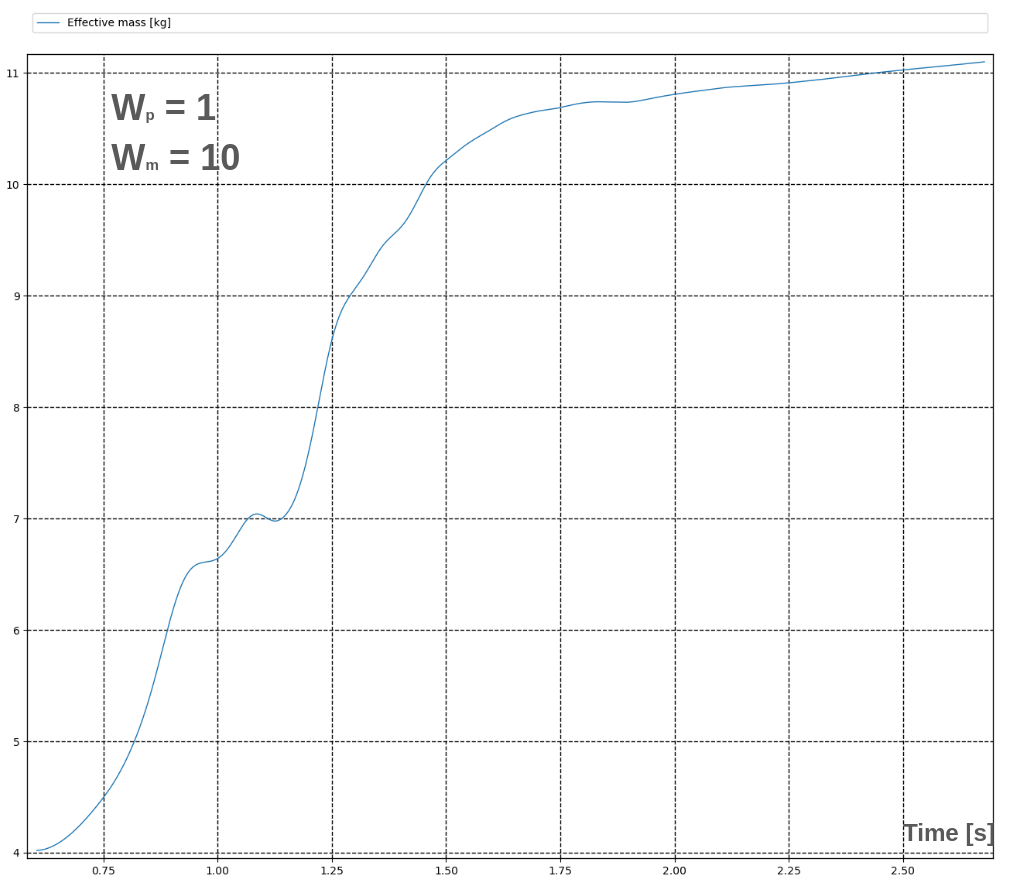
\includegraphics[width=0.9\linewidth]{EMMT_1_10.png}
%     \caption{Time evolution of the EMR, $W_p = 1, W_m = 10$}
%     \label{Time evolution of the effective mass of the robot 2}
% \end{figure}
% \noindent
Then, we use BSTT and VOT, which are already implemented in mc\_rtc and we display the tracking of the theoretical trajectory given by the Bézier curve (\ref{Bézier curve}), with the following curve constraints: 
$\bm {\kappa}_{\mathbf{\dot x}_{\nu}^{t_i}} = (0, 0, 0)^\mathbf{T}$ 
$,
\bm {\kappa}_{\mathbf{\ddot x}_{\nu}^{t_i}} = (0, 0, 0)^\mathbf{T}
$,
$
\bm {\kappa}_{\mathbf{\ddot x}_{\nu}^{t_c}} = (0, 0, 0)^\mathbf{T}
$, and especially
\begin{equation}
 % \bm {\kappa}_{\mathbf{\dot x}_{\nu}^{t_c}} = {V_{f,in}^w} \mathbf{n}_w
 \bm {\kappa}_{\mathbf{\dot x}_{\nu}^{t_c}} = \mathbf{R}_{w \to nail}^{\mathbf{T}} {}^{nail}\mathbf{\dot x}_{\nu}^{t_c} 
\end{equation}
% where ${V_{f,in}^w} \in \mathbb{R}$ is the input final velocity on the nail expressed in the world frame $w$, in meters per second.
where ${{}^{nail}\mathbf{\dot x}_{\nu}^{t_c}} \in \mathbb{R}^3$ is the input velocity of the hammer tip at the instant of contact $t_c$ expressed in the nail frame. 
The nail is placed at $\mathbf{c}^{nail} = (0.75, 0.40, 0.90)^\mathbf{T}$ from the origin of $w$ with the distances given in meters, and oriented as depicted by Fig.~\ref{SCHEMATIC OF THE PROBLEM}, i.e perpendicular to an horizontal plane. 
We set $T = 1$s, $W_{B} = 100$, $W_{VOT} = 10$, $W_{m} = 100$, $W_{p} = 1$, ${}^{nail}\mathbf{\dot x}_{\nu}^{t_c} = (0, 0 ,  -2.0) ^\mathbf{T}$ m/s, the stiffness of the BSTT to $K_{p, B} = 10000$ and the stiffness of the VOT to $K_{p, VOT} = 1000$ with their damping given by (\ref{Kp Kd relationship}). 
We see the tracking of the hammer tip velocity in Fig.~\ref{Velocity tracking of the hammer tip}(a). 
It is worth to mention that the hammer tip properly reaches ${}^{nail}\mathbf{\dot x}_{\nu}^{t_c}$ until the sudden spike in velocity at the end, which is due to a collision with the nail. 
However, we also see some unwanted oscillations on the $z$ coordinate: this is due to the high stiffness ($1000$) of the VOT. 
The final orientation error has been recorded to be $4.16$ deg. 
We decrease the stiffness of the VOT to 250 in Fig.~\ref{Velocity tracking of the hammer tip}(b) and we record an orientation error of $11.88$ deg. 
Increasing $K_{p, VOT}$ decreases the error between the desired and actual final hammer tip orientations at the cost of larger oscillations at the beginning.
The projected momentum of the hammer tip is computed using (\ref{Momentum end effector}) and is shown in Fig.~\ref{Time evolution of the momentum projected along the normal n}, 
with the impulse displayed with the sudden jump in projected momentum. 
% \begin{figure}
%     \centering
%     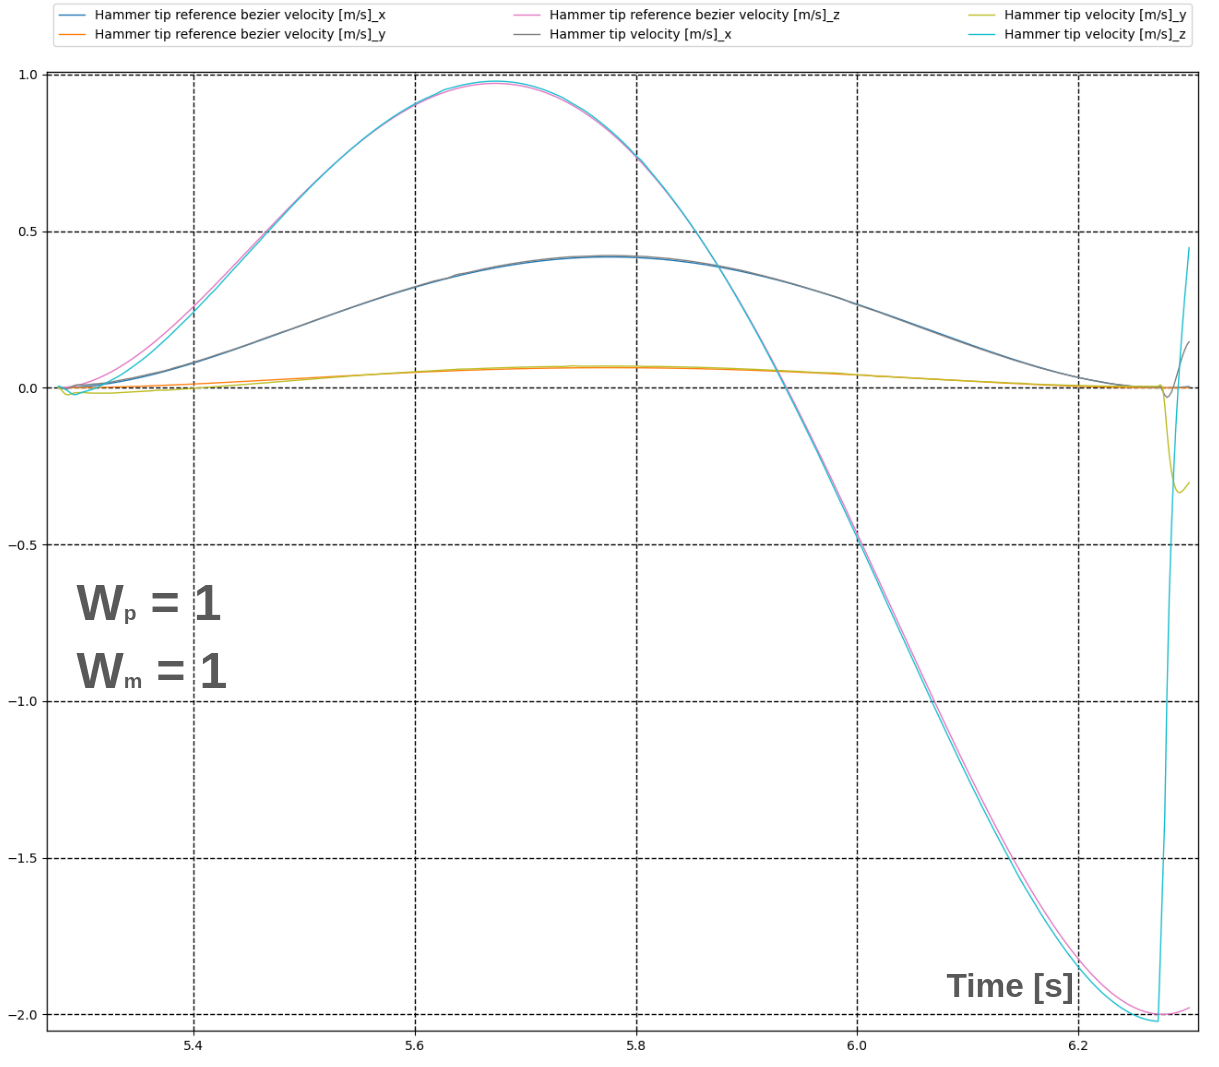
\includegraphics[width=0.85\linewidth]{Velocity graph.png}
%     \caption{Velocity tracking of the hammer tip}
%     \label{Velocity tracking of the hammer tip}
% \end{figure}
% \begin{figure}
%     \centering
%     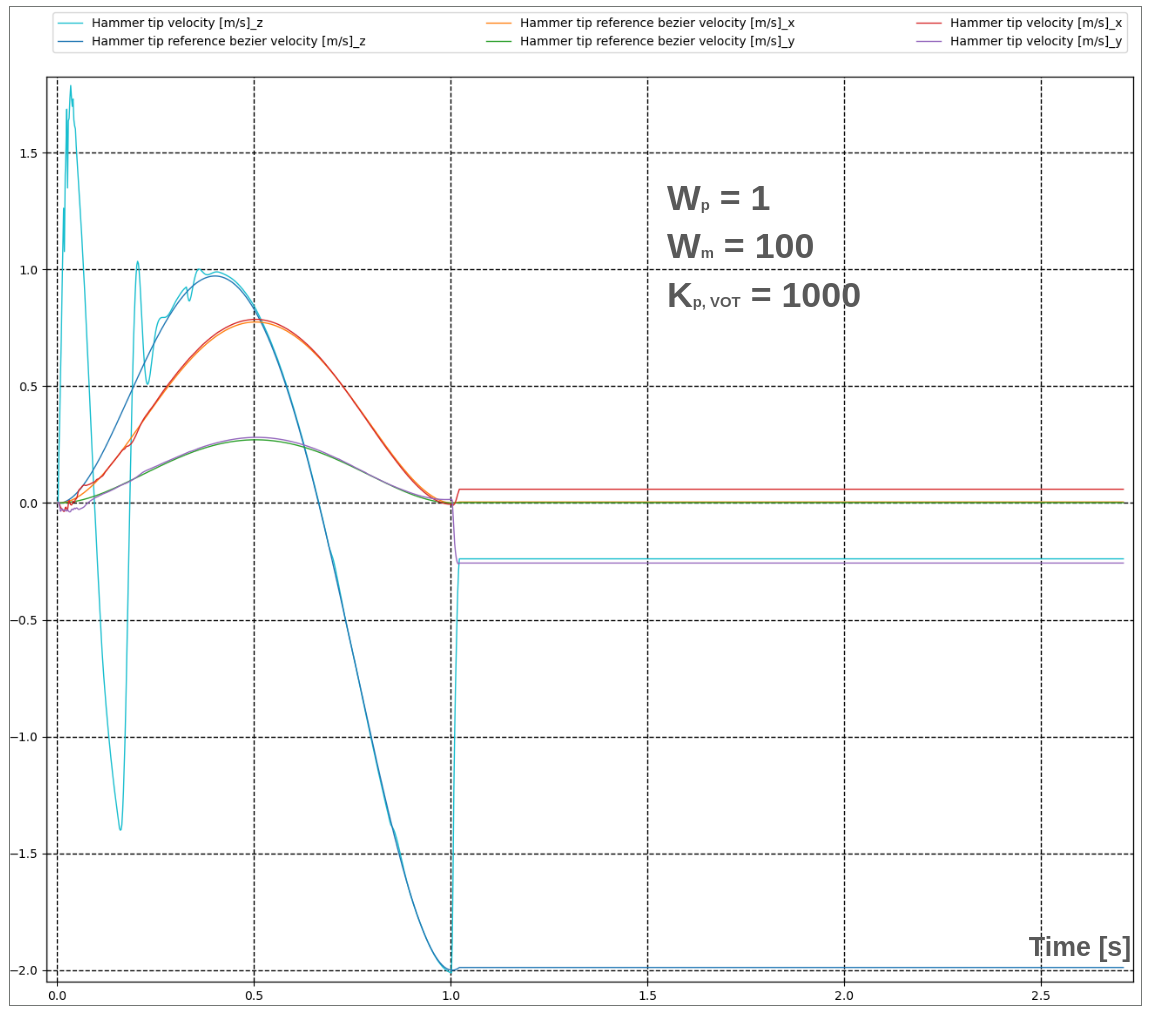
\includegraphics[width=0.75\linewidth]{Velocity with VOT.png}
%     \caption{Velocity tracking of the hammer tip, $K_{p, VOT} = 1000$}
%     \label{Velocity tracking of the hammer tip}
% \end{figure}
% \begin{figure}
%     \centering
%     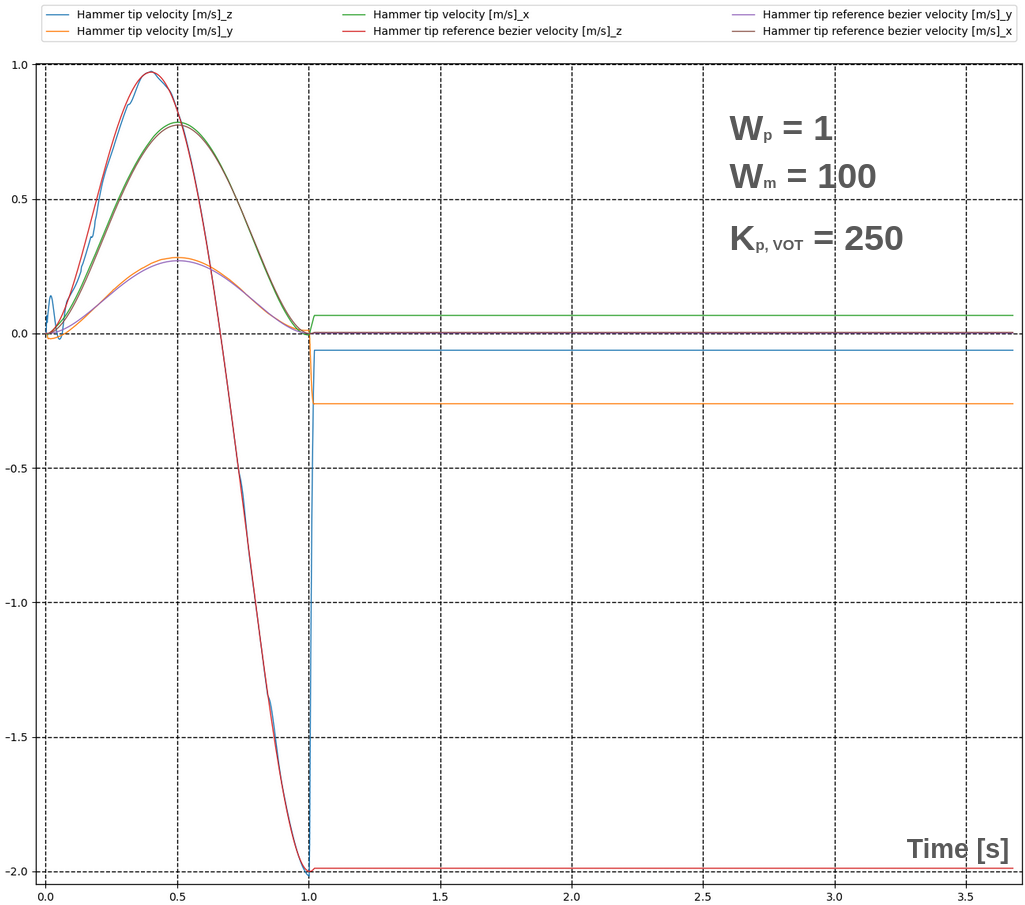
\includegraphics[width=0.75\linewidth]{Velocity graph VOT 250.png}
%     \caption{Velocity tracking of the hammer tip, $K_{p, VOT} = 250$}
%     \label{Velocity tracking of the hammer tip, $K_{p,VOT} = 250$}
% \end{figure}


% \begin{figure}
%     \centering
%     \includegraphics[width=0.75\linewidth]{Velocity graph with VOT.png}
%     \caption{Velocity tracking of the hammer tip}
%     \label{Velocity tracking of the hammer tip}
% \end{figure}
\section{Conclusion}
\noindent
In this work, we presented a way to implement a hammering task on a humanoid robot. 
% We used a momentum based model to estimate the dynamics of the robot and the nail after impact. 
We proposed our method to maximize the EMR using its gradient and QP, then we suggested an end-effector trajectory built from a constrained $5^{th}$ order Bézier curve. 
Simulations showed that the EMR is getting maximized and the trajectory given by the Bézier curve is properly followed by the end-effector. 

Possible improvements include an estimation of the nail penetration in an object (like a wood table) along with a simulation of the dynamics of the nail, a way to build our path and orientation to the nail by efficiently considering collision constraints with the environment or a post-impact reference that utilizes the post-impact velocity of the hammer tip to prepare for the next hit, as the robot only goes back to its initial posture for now. 

In the future, we want to work on the stability problem of the robot potentially induced by the post-impact rebounce of the hammer, on minimizing the damage that the robot must endure on its joints and on detection of the nail via computer vision. 
\label{Conclusion}

% \section{Prepare Your Paper Before Styling}
% Before you begin to format your paper, first write and save the content as a 
% separate text file. Complete all content and organizational editing before 
% formatting. Please note sections \ref{AA}--\ref{SCM} below for more information on 
% proofreading, spelling and grammar.

% Keep your text and graphic files separate until after the text has been 
% formatted and styled. Do not number text heads---{\LaTeX} will do that 
% for you.

% \subsection{Abbreviations and Acronyms}\label{AA}
% Define abbreviations and acronyms the first time they are used in the text, 
% even after they have been defined in the abstract. Abbreviations such as 
% IEEE, SI, MKS, CGS, ac, dc, and rms do not have to be defined. Do not use 
% abbreviations in the title or heads unless they are unavoidable.

% \subsection{Units}
% \begin{itemize}
% \item Use either SI (MKS) or CGS as primary units. (SI units are encouraged.) English units may be used as secondary units (in parentheses). An exception would be the use of English units as identifiers in trade, such as ``3.5-inch disk drive''.
% \item Avoid combining SI and CGS units, such as current in amperes and magnetic field in oersteds. This often leads to confusion because equations do not balance dimensionally. If you must use mixed units, clearly state the units for each quantity that you use in an equation.
% \item Do not mix complete spellings and abbreviations of units: ``Wb/m\textsuperscript{2}'' or ``webers per square meter'', not ``webers/m\textsuperscript{2}''. Spell out units when they appear in text: ``. . . a few henries'', not ``. . . a few H''.
% \item Use a zero before decimal points: ``0.25'', not ``.25''. Use ``cm\textsuperscript{3}'', not ``cc''.)
% \end{itemize}

% \subsection{Equations}
% Number equations consecutively. To make your 
% equations more compact, you may use the solidus (~/~), the exp function, or 
% appropriate exponents. Italicize Roman symbols for quantities and variables, 
% but not Greek symbols. Use a long dash rather than a hyphen for a minus 
% sign. Punctuate equations with commas or periods when they are part of a 
% sentence, as in:
% \begin{equation}
% a+b=\gamma\label{eq}
% \end{equation}

% Be sure that the 
% symbols in your equation have been defined before or immediately following 
% the equation. Use ``\eqref{eq}'', not ``Eq.~\eqref{eq}'' or ``equation \eqref{eq}'', except at 
% the beginning of a sentence: ``Equation \eqref{eq} is . . .''

% \subsection{\LaTeX-Specific Advice}

% Please use ``soft'' (e.g., \verb|\eqref{Eq}|) cross references instead
% of ``hard'' references (e.g., \verb|(1)|). That will make it possible
% to combine sections, add equations, or change the order of figures or
% citations without having to go through the file line by line.

% Please don't use the \verb|{eqnarray}| equation environment. Use
% \verb|{align}| or \verb|{IEEEeqnarray}| instead. The \verb|{eqnarray}|
% environment leaves unsightly spaces around relation symbols.

% Please note that the \verb|{subequations}| environment in {\LaTeX}
% will increment the main equation counter even when there are no
% equation numbers displayed. If you forget that, you might write an
% article in which the equation numbers skip from (17) to (20), causing
% the copy editors to wonder if you've discovered a new method of
% counting.

% {\BibTeX} does not work by magic. It doesn't get the bibliographic
% data from thin air but from .bib files. If you use {\BibTeX} to produce a
% bibliography you must send the .bib files. 

% {\LaTeX} can't read your mind. If you assign the same label to a
% subsubsection and a table, you might find that Table I has been cross
% referenced as Table IV-B3. 

% {\LaTeX} does not have precognitive abilities. If you put a
% \verb|\label| command before the command that updates the counter it's
% supposed to be using, the label will pick up the last counter to be
% cross referenced instead. In particular, a \verb|\label| command
% should not go before the caption of a figure or a table.

% Do not use \verb|\nonumber| inside the \verb|{array}| environment. It
% will not stop equation numbers inside \verb|{array}| (there won't be
% any anyway) and it might stop a wanted equation number in the
% surrounding equation.

% \subsection{Some Common Mistakes}\label{SCM}
% \begin{itemize}
% \item The word ``data'' is plural, not singular.
% \item The subscript for the permeability of vacuum $\mu_{0}$, and other common scientific constants, is zero with subscript formatting, not a lowercase letter ``o''.
% \item In American English, commas, semicolons, periods, question and exclamation marks are located within quotation marks only when a complete thought or name is cited, such as a title or full quotation. When quotation marks are used, instead of a bold or italic typeface, to highlight a word or phrase, punctuation should appear outside of the quotation marks. A parenthetical phrase or statement at the end of a sentence is punctuated outside of the closing parenthesis (like this). (A parenthetical sentence is punctuated within the parentheses.)
% \item A graph within a graph is an ``inset'', not an ``insert''. The word alternatively is preferred to the word ``alternately'' (unless you really mean something that alternates).
% \item Do not use the word ``essentially'' to mean ``approximately'' or ``effectively''.
% \item In your paper title, if the words ``that uses'' can accurately replace the word ``using'', capitalize the ``u''; if not, keep using lower-cased.
% \item Be aware of the different meanings of the homophones ``affect'' and ``effect'', ``complement'' and ``compliment'', ``discreet'' and ``discrete'', ``principal'' and ``principle''.
% \item Do not confuse ``imply'' and ``infer''.
% \item The prefix ``non'' is not a word; it should be joined to the word it modifies, usually without a hyphen.
% \item There is no period after the ``et'' in the Latin abbreviation ``et al.''.
% \item The abbreviation ``i.e.'' means ``that is'', and the abbreviation ``e.g.'' means ``for example''.
% \end{itemize}
% An excellent style manual for science writers is \cite{b7}.

% \subsection{Authors and Affiliations}
% \textbf{The class file is designed for, but not limited to, six authors.} A 
% minimum of one author is required for all conference articles. Author names 
% should be listed starting from left to right and then moving down to the 
% next line. This is the author sequence that will be used in future citations 
% and by indexing services. Names should not be listed in columns nor group by 
% affiliation. Please keep your affiliations as succinct as possible (for 
% example, do not differentiate among departments of the same organization).

% \subsection{Identify the Headings}
% Headings, or heads, are organizational devices that guide the reader through 
% your paper. There are two types: component heads and text heads.

% Component heads identify the different components of your paper and are not 
% topically subordinate to each other. Examples include Acknowledgments and 
% References and, for these, the correct style to use is ``Heading 5''. Use 
% ``figure caption'' for your Figure captions, and ``table head'' for your 
% table title. Run-in heads, such as ``Abstract'', will require you to apply a 
% style (in this case, italic) in addition to the style provided by the drop 
% down menu to differentiate the head from the text.

% Text heads organize the topics on a relational, hierarchical basis. For 
% example, the paper title is the primary text head because all subsequent 
% material relates and elaborates on this one topic. If there are two or more 
% sub-topics, the next level head (uppercase Roman numerals) should be used 
% and, conversely, if there are not at least two sub-topics, then no subheads 
% should be introduced.

% \subsection{Figures and Tables}
% \paragraph{Positioning Figures and Tables} Place figures and tables at the top and 
% bottom of columns. Avoid placing them in the middle of columns. Large 
% figures and tables may span across both columns. Figure captions should be 
% below the figures; table heads should appear above the tables. Insert 
% figures and tables after they are cited in the text. Use the abbreviation 
% ``Fig.~\ref{fig}'', even at the beginning of a sentence.

% \begin{table}[htbp]
% \caption{Table Type Styles}
% \begin{center}
% \begin{tabular}{|c|c|c|c|}
% \hline
% \textbf{Table}&\multicolumn{3}{|c|}{\textbf{Table Column Head}} \\
% \cline{2-4} 
% \textbf{Head} & \textbf{\textit{Table column subhead}}& \textbf{\textit{Subhead}}& \textbf{\textit{Subhead}} \\
% \hline
% copy& More table copy$^{\mathrm{a}}$& &  \\
% \hline
% \multicolumn{4}{l}{$^{\mathrm{a}}$Sample of a Table footnote.}
% \end{tabular}
% \label{tab1}
% \end{center}
% \end{table}

% \begin{figure}[htbp]
% \centerline{\includegraphics{fig1.png}}
% \caption{Example of a figure caption.}
% \label{fig}
% \end{figure}

% Figure Labels: Use 8 point Times New Roman for Figure labels. Use words 
% rather than symbols or abbreviations when writing Figure axis labels to 
% avoid confusing the reader. As an example, write the quantity 
% ``Magnetization'', or ``Magnetization, M'', not just ``M''. If including 
% units in the label, present them within parentheses. Do not label axes only 
% with units. In the example, write ``Magnetization (A/m)'' or ``Magnetization 
% \{A[m(1)]\}'', not just ``A/m''. Do not label axes with a ratio of 
% quantities and units. For example, write ``Temperature (K)'', not 
% ``Temperature/K''.

% \section*{Acknowledgment}

% The preferred spelling of the word ``acknowledgment'' in America is without 
% an ``e'' after the ``g''. Avoid the stilted expression ``one of us (R. B. 
% G.) thanks $\ldots$''. Instead, try ``R. B. G. thanks$\ldots$''. Put sponsor 
% acknowledgments in the unnumbered footnote on the first page.

% % \begin{equation}
% %     m_{e,\mathbf{n}} = \left(\mathbf{n^T \bm \Lambda n}\right)^{-1}
% % \end{equation}
% % \begin{equation} 
% %     \bm \Lambda = \mathbf{J_\nu M^{-1}J_\nu^T} 
% % \end{equation}
% % \begin{equation}
% %     m_{e,\mathbf{n}} = \mathbf{n^T \bm \Lambda_\nu^{-1} n}
% % \end{equation}
% % \begin{equation}
% %     \bm \Lambda_\nu = \left(\mathbf{J_\nu M^{-1}J_\nu^T}\right)^{-1} 
% % \end{equation}
% \section*{References}

% Please number citations consecutively within brackets \cite{b1}. The 
% sentence punctuation follows the bracket \cite{b2}. Refer simply to the reference 
% number, as in \cite{b3}---do not use ``Ref. \cite{b3}'' or ``reference \cite{b3}'' except at 
% the beginning of a sentence: ``Reference \cite{b3} was the first $\ldots$''

% Number footnotes separately in superscripts. Place the actual footnote at 
% the bottom of the column in which it was cited. Do not put footnotes in the 
% abstract or reference list. Use letters for table footnotes.

% Unless there are six authors or more give all authors' names; do not use 
% ``et al.''. Papers that have not been published, even if they have been 
% submitted for publication, should be cited as ``unpublished'' \cite{b4}. Papers 
% that have been accepted for publication should be cited as ``in press'' \cite{b5}. 
% Capitalize only the first word in a paper title, except for proper nouns and 
% element symbols.

% For papers published in translation journals, please give the English 
% citation first, followed by the original foreign-language citation \cite{b6}.
\section*{Acknowledgment}
\noindent
This research was funded by JSPS KAKENHI, grant number 24K00836.
\printbibliography
% \begin{thebibliography}{00}
% \bibitem{b1} G. Eason, B. Noble, and I. N. Sneddon, ``On certain integrals of Lipschitz-Hankel type involving products of Bessel functions,'' Phil. Trans. Roy. Soc. London, vol. A247, pp. 529--551, April 1955.
% \bibitem{b2} J. Clerk Maxwell, A Treatise on Electricity and Magnetism, 3rd ed., vol. 2. Oxford: Clarendon, 1892, pp.68--73.
% \bibitem{b3} I. S. Jacobs and C. P. Bean, ``Fine particles, thin films and exchange anisotropy,'' in Magnetism, vol. III, G. T. Rado and H. Suhl, Eds. New York: Academic, 1963, pp. 271--350.
% \bibitem{b4} K. Elissa, ``Title of paper if known,'' unpublished.
% \bibitem{b5} R. Nicole, ``Title of paper with only first word capitalized,'' J. Name Stand. Abbrev., in press.
% \bibitem{b6} Y. Yorozu, M. Hirano, K. Oka, and Y. Tagawa, ``Electron spectroscopy studies on magneto-optical media and plastic substrate interface,'' IEEE Transl. J. Magn. Japan, vol. 2, pp. 740--741, August 1987 [Digests 9th Annual Conf. Magnetics Japan, p. 301, 1982].
% \bibitem{b7} M. Young, The Technical Writer's Handbook. Mill Valley, CA: University Science, 1989.
% \end{thebibliography}
% \vspace{12pt}
% \color{red}
% IEEE conference templates contain guidance text for composing and formatting conference papers. Please ensure that all template text is removed from your conference paper prior to submission to the conference. Failure to remove the template text from your paper may result in your paper not being published.

\end{document}


